%=============================================================================
%  CHAPTER 2 — ANALYSIS AND SPECIFICATION OF REQUIREMENTS
%=============================================================================
\chapter{Analysis and Specification of Requirements}

\clearpage
\section*{Introduction}

The previous chapter established the context of the project and stated the high-level objectives of ForsaDrive. The present chapter takes the analysis one step further by clarifying, in a structured way, who the platform is for, what it must do, and what quality attributes it must respect. The reasoning starts with a comparative review of the mobility solutions on which Tunisians currently rely, ranging from informal social-media groups to international ride-hailing applications. It continues with the description of the development methodology adopted throughout the internship, the identification of the actors of the system, and the listing of the functional and non-functional requirements. The chapter closes with a global use case diagram that summarizes the scope of the platform and prepares the conception phase presented in the next chapter.


\section{Study of Existing Solutions}

Before designing ForsaDrive, it was essential to understand how Tunisians currently organize shared trips, both through formal applications and through informal channels. This step served two complementary purposes: it allowed an objective measure of the gaps left by existing tools and it informed several design decisions presented later, such as the combination of online prepayment and cash settlement.

\subsection{Informal Carpooling through Social Media}

A large share of carpooling activity in Tunisia takes place outside any structured platform. Facebook groups such as \textit{Covoiturage Tunisie}, \textit{Covoiturage Tunis--Sfax}, and regional groups dedicated to specific universities are among the most active channels. Trips are published as simple posts, and passengers contact drivers through private messages or phone calls.

While this informal system genuinely meets part of the demand, it suffers from several structural weaknesses:

\begin{itemize}[noitemsep]
    \item There is no verification of the identity of the driver or of the vehicle.
    \item Payments are handled entirely offline, with no trace of the transaction.
    \item Trip information is scattered across several groups, and no real filtering or sorting is possible.
    \item Cancellations and no-shows are frequent, since neither party has any concrete commitment.
    \item There is no rating system, which forces passengers to rely solely on the comments left under each post.
\end{itemize}

This mode of organization is tolerated rather than regulated, and its very popularity illustrates how strong the demand is for a structured digital alternative.

\begin{figure}[H]
    \centering
    
\includegraphics[width=0.7\textwidth]{Post covoiturage.png}
    \caption{Example of an informal carpooling post on a Facebook group}
    \label{fig:facebook_carpooling}
\end{figure}

\subsection{International Ride-Hailing Applications}

Several international ride-hailing applications are currently active on the Tunisian market. Although they are not carpooling platforms in the strict sense, they are often mentioned by users as alternatives for point-to-point travel, which justifies their inclusion in this comparative study.

\subsubsection{inDrive}
inDrive is built on a fare-negotiation model: the passenger proposes a price and drivers can accept the offer or counter-offer. The application is mainly used inside cities such as Tunis, Sousse, and Sfax. However, inDrive is not designed for long-distance travel. Its pricing logic becomes impractical for inter-city routes, and drivers have very little incentive to accept negotiated long trips at a price they cannot adjust based on the number of passengers sharing the vehicle.

\begin{figure}[H]
    \centering
    
\includegraphics[width=0.3\textwidth]{img/indrive.png}
    \caption{inDrive logo}
    \label{fig:indrive_logo}
\end{figure}

\subsubsection{Bolt}
Bolt operates as a classic ride-hailing service with fixed, algorithmic pricing. It is widely used for short urban trips, but it offers no mechanism for sharing a vehicle between passengers heading in the same direction, and its fares rise sharply on longer journeys, which excludes inter-city carpooling from its use cases.

\begin{figure}[H]
    \centering
    
\includegraphics[width=0.3\textwidth]{img/bolt_logo.png}
    \caption{Bolt logo}
    \label{fig:bolt_logo}
\end{figure}

\subsubsection{Uber}
Uber has only a limited presence in Tunisia and is essentially absent from the inter-city segment. For the use cases targeted by ForsaDrive, it is therefore not a realistic alternative.

\subsection{International Carpooling Platforms}

BlaBlaCar is the most well-known carpooling platform internationally and is also used, although on a modest scale, in Tunisia. It offers a structured experience built around verified profiles, integrated payments, and ratings. Its adoption in Tunisia, however, remains low for reasons that have little to do with the quality of the platform itself: payment methods are mostly limited to international cards, customer support operates in foreign languages, and the local user base is too small to ensure frequent matches on the most requested national routes. As a result, the value of the network — which is the main strength of carpooling platforms — is significantly reduced in the Tunisian context.

\begin{figure}[H]
    \centering
    
\includegraphics[width=0.3\textwidth]{img/blablacar.png}
    \caption{BlaBlaCar logo}
    \label{fig:blablacar_logo}
\end{figure}

\subsection{Comparative Table}

Table~\ref{tab:comparison_existing} summarizes the main characteristics of the solutions reviewed above and contrasts them with the features targeted by ForsaDrive.

\begin{table}[H]
\centering
\caption{Comparison of existing solutions with ForsaDrive}
\label{tab:comparison_existing}
\begin{tabular}{|l|c|c|c|c|c|}
\hline
\textbf{Criterion}       & \textbf{Facebook} & \textbf{inDrive} & \textbf{Bolt} & \textbf{BlaBlaCar} & \textbf{ForsaDrive} \\
\hline
Identity verification    & No  & Partial & Yes & Yes & Yes \\
\hline
In-app payment           & No  & No      & Yes & Yes & Yes \\
\hline
Long-distance rides      & Yes & No      & No  & Yes & Yes \\
\hline
Rating system            & No  & Yes     & Yes & Yes & Yes \\
\hline
Adapted to local context & Yes & Partial & Partial & No & Yes \\
\hline
Student discount         & No  & No      & No  & No & Yes \\
\hline
Wallet-based balance     & No  & No      & No  & No & Yes \\
\hline
\end{tabular}
\end{table}

The analysis shows that no existing option simultaneously offers the local fit of informal channels and the reliability of structured platforms. ForsaDrive is positioned precisely in this gap, combining the familiarity of practices that Tunisian users already adopt with the structure, security, and trust mechanisms that international platforms have demonstrated elsewhere.


\section{Development Methodology}

\subsection{Choice of an Agile Approach}

Given the scope of the project, which combines a web application, a mobile application, and a shared backend, a sequential approach such as the waterfall model was rapidly ruled out. Several reasons supported this decision. First, the requirements were expected to evolve as the design progressed, which is typical for a platform whose features have direct counterparts in the daily life of the target users. Second, the project required iterative feedback with the supervising team at ATOMIC IT in order to validate design choices step by step. Third, the team was small and the schedule short, two conditions under which the lightness of an agile process is a clear advantage over the heavier ceremonies of more formal methodologies. The \textbf{Scrum} framework was therefore selected as the development methodology of the project.

\subsection{The Scrum Framework}

Scrum organizes the work into short iterations called sprints, each of which produces a usable increment of the product. Every sprint is planned at the beginning, reviewed at the end, and followed by a short retrospective whose role is to identify what worked, what did not, and which adjustments to apply during the next iteration. Three roles structure the process: the \textit{Product Owner}, who represents the client and maintains the prioritized backlog; the \textit{Scrum Master}, who facilitates the process and removes blocking issues; and the \textit{Development Team}, which builds the increment.

\begin{figure}[H]
    \centering
    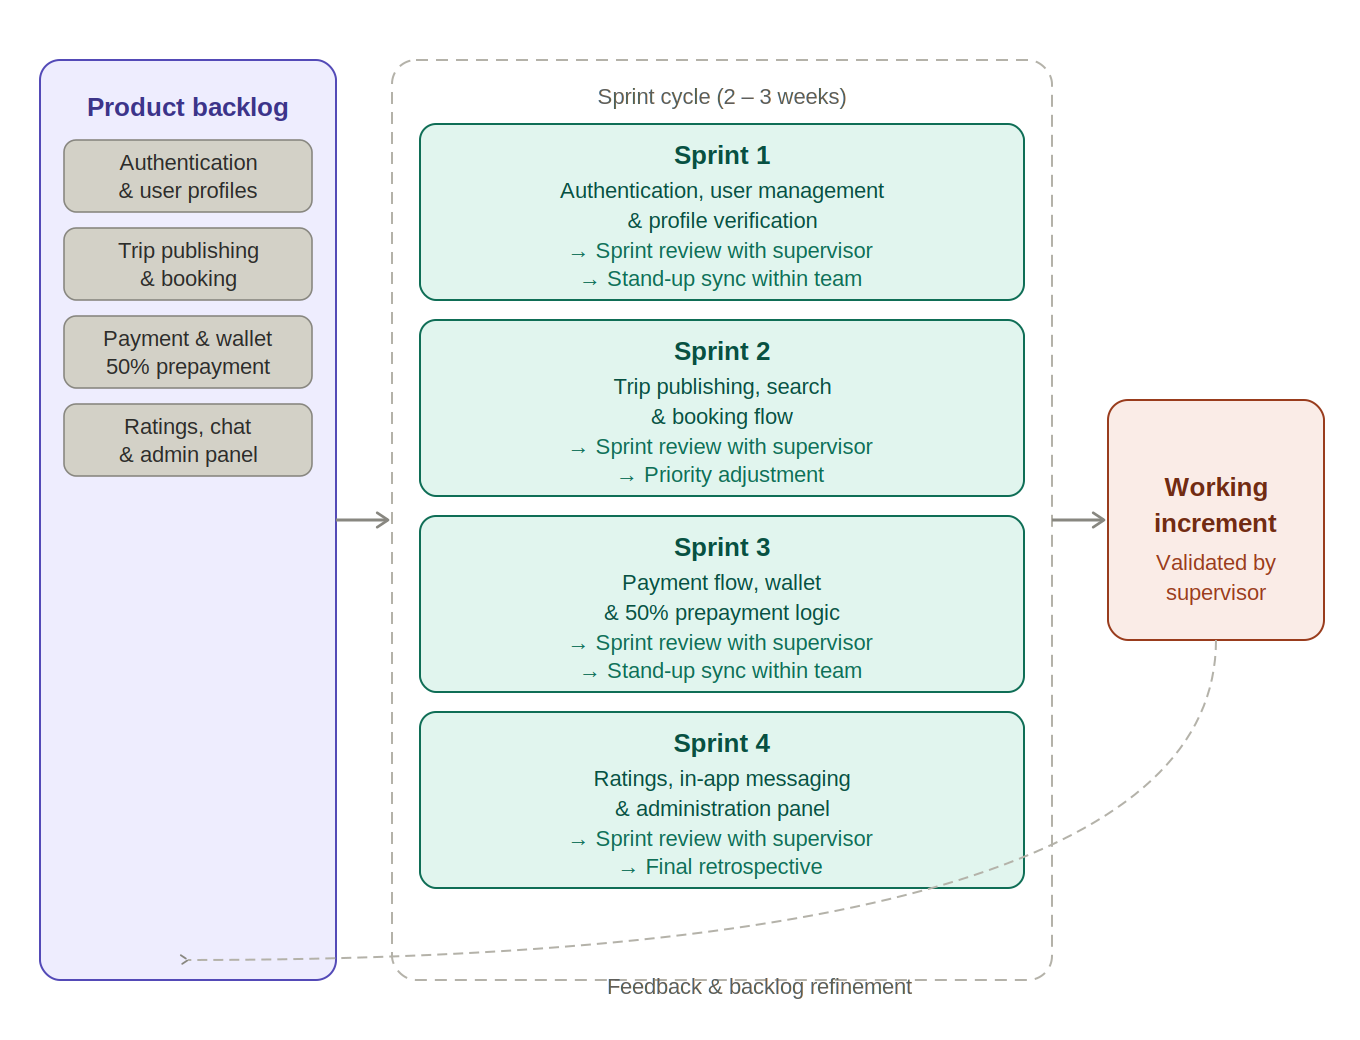
\includegraphics[width=0.9\textwidth]{forsadrive_scrum.png}
    \caption{Overview of the Scrum framework}
    \label{fig:scrum_framework}
\end{figure}

\subsection{Application to ForsaDrive}

In the context of this internship, Scrum was applied in a simplified form adapted to a two-student team. The work was organized into four functional sprints, each of which produced a coherent increment of the platform.

\begin{enumerate}[noitemsep]
    \item \textbf{Sprint 1 — Foundations.} Project setup, authentication, profile management, role management, student verification, driver profile creation, and administrative validation.
    \item \textbf{Sprint 2 — Rides and Bookings.} Ride publishing, search and filtering, single and group bookings, and management of booking requests.
    \item \textbf{Sprint 3 — Payments and Intelligence.} Wallet, fifty-percent prepayment, student discount calculation, ride boosting, driver analytics, and recommendation logic.
    \item \textbf{Sprint 4 — Community and Finalization.} In-app messaging, ratings, complaint handling, social feed, HelpDesk, multilingual support, testing, and deployment.
\end{enumerate}

Short stand-up meetings were held inside the team to coordinate the day-to-day work, and weekly reviews were organized with the supervising engineer to validate progress and adjust priorities. This rhythm proved well suited to a project of this size, since it kept the team focused on a small set of features at a time while preserving the flexibility needed to absorb changes coming from the reviews.


\section{Identification of Actors}

In the UML sense, an actor is any entity, human or automated, that interacts with the system. Four human actors and one automated actor were identified for ForsaDrive.

\begin{description}[noitemsep]
    \item[Guest.] An unauthenticated visitor who can browse the public landing page, consult general information about the platform, and start the registration process.
    \item[Passenger.] A registered user looking for a trip. A passenger can search for available rides, book seats, pay the prepayment, communicate with the driver, and rate the trip after its completion.
    \item[Driver.] A registered user who offers trips. A driver can create, modify, or cancel rides, accept or decline booking requests, and receive payments through the platform.
    \item[Administrator.] The operator of the platform. The administrator is responsible for verifying user identities, validating student documents, moderating reported content, handling disputes, and supervising the overall activity of the platform.
    \item[System.] An automated actor that triggers operations such as the calculation of the student discount, the dispatch of notifications, and the recomputation of the reliability score after each completed trip.
\end{description}

The role of \textit{Student} is not modeled as a separate actor but as a status attached to a passenger account. This status is granted after a successful verification process and gives access to the fifty-percent discount on eligible trips.


\section{Functional Requirements}

Functional requirements describe what the system must do. They are grouped here by actor in order to reflect the structure of the use case diagram presented at the end of the chapter.

\subsection{Requirements for the Guest}

\begin{itemize}[noitemsep]
    \item Browse the public landing page and consult general information about the platform.
    \item Register a new account, choosing between a passenger and a driver role.
    \item Authenticate through email and password.
    \item Recover a forgotten password through a secure procedure.
\end{itemize}

\subsection{Requirements for the Passenger}

\begin{itemize}[noitemsep]
    \item Search for trips by departure city, arrival city, and date.
    \item Filter results by price, departure time, and driver rating.
    \item Consult the full details of a trip, including the profile of the driver.
    \item Reserve one or several seats on a trip.
    \item Pay fifty percent of the amount as a prepayment at the moment of booking.
    \item Benefit from the student discount once the account is verified as such.
    \item Cancel a booking under the cancellation rules defined by the platform.
    \item Rate and review a driver after a completed trip.
    \item Exchange messages with a driver through the in-app chat.
\end{itemize}

\subsection{Requirements for the Driver}

\begin{itemize}[noitemsep]
    \item Publish a new trip with its origin, destination, date, time, price, and number of available seats.
    \item Modify or cancel an existing trip while respecting the rules that protect already booked passengers.
    \item View and manage incoming booking requests.
    \item Access a wallet that summarizes earned, pending, and refunded amounts.
    \item Receive notifications about new bookings and incoming messages.
    \item Rate a passenger after a completed trip.
\end{itemize}

\subsection{Requirements for the Administrator}

\begin{itemize}[noitemsep]
    \item Authenticate through a dedicated administration panel.
    \item Manage user accounts (activation, deactivation, verification).
    \item Review and validate identity documents and student cards.
    \item Moderate reported trips, users, or messages.
    \item Consult global statistics on users, trips, and payments.
\end{itemize}


\section{Non-Functional Requirements}

Non-functional requirements describe the quality attributes that the system must respect. They constrain the design as much as the functional requirements do, since they directly affect the trust that users place in the platform.

\begin{description}[noitemsep]
    \item[Security.] Authentication relies on hashed passwords. Sensitive operations such as payment and account modification require an active and validated session. All exchanges between client and server are protected by HTTPS, and identity documents are stored in a dedicated, access-controlled location.
    \item[Performance.] The system must remain responsive under normal load. Search results, in particular, must be returned within a delay short enough to preserve a fluid user experience.
    \item[Availability.] The platform must remain reachable at all times, except during scheduled maintenance windows announced in advance to the users.
    \item[Usability.] The interfaces are clear and consistent across the web and mobile platforms. A new user must be able to book a trip without external assistance, which requires careful attention to information density, form validation, and feedback messages.
    \item[Portability.] The mobile application runs on recent versions of Android and iOS. The web application is compatible with the major modern browsers.
    \item[Scalability.] The architecture allows new features to be added without rewriting existing modules. This is particularly important for ForsaDrive, since the roadmap includes intelligent services that will be plugged into the existing booking workflow.
    \item[Maintainability.] The source code follows clear conventions and a layered organization, so that a new contributor can become productive within a reasonable amount of time.
\end{description}


\section{Global Use Case Diagram}

The global use case diagram synthesizes the main interactions between the actors and the system. It provides the first complete view of the functional coverage of ForsaDrive and serves as the entry point for the conception phase of the next chapter.

\begin{figure}[H]
    \centering
    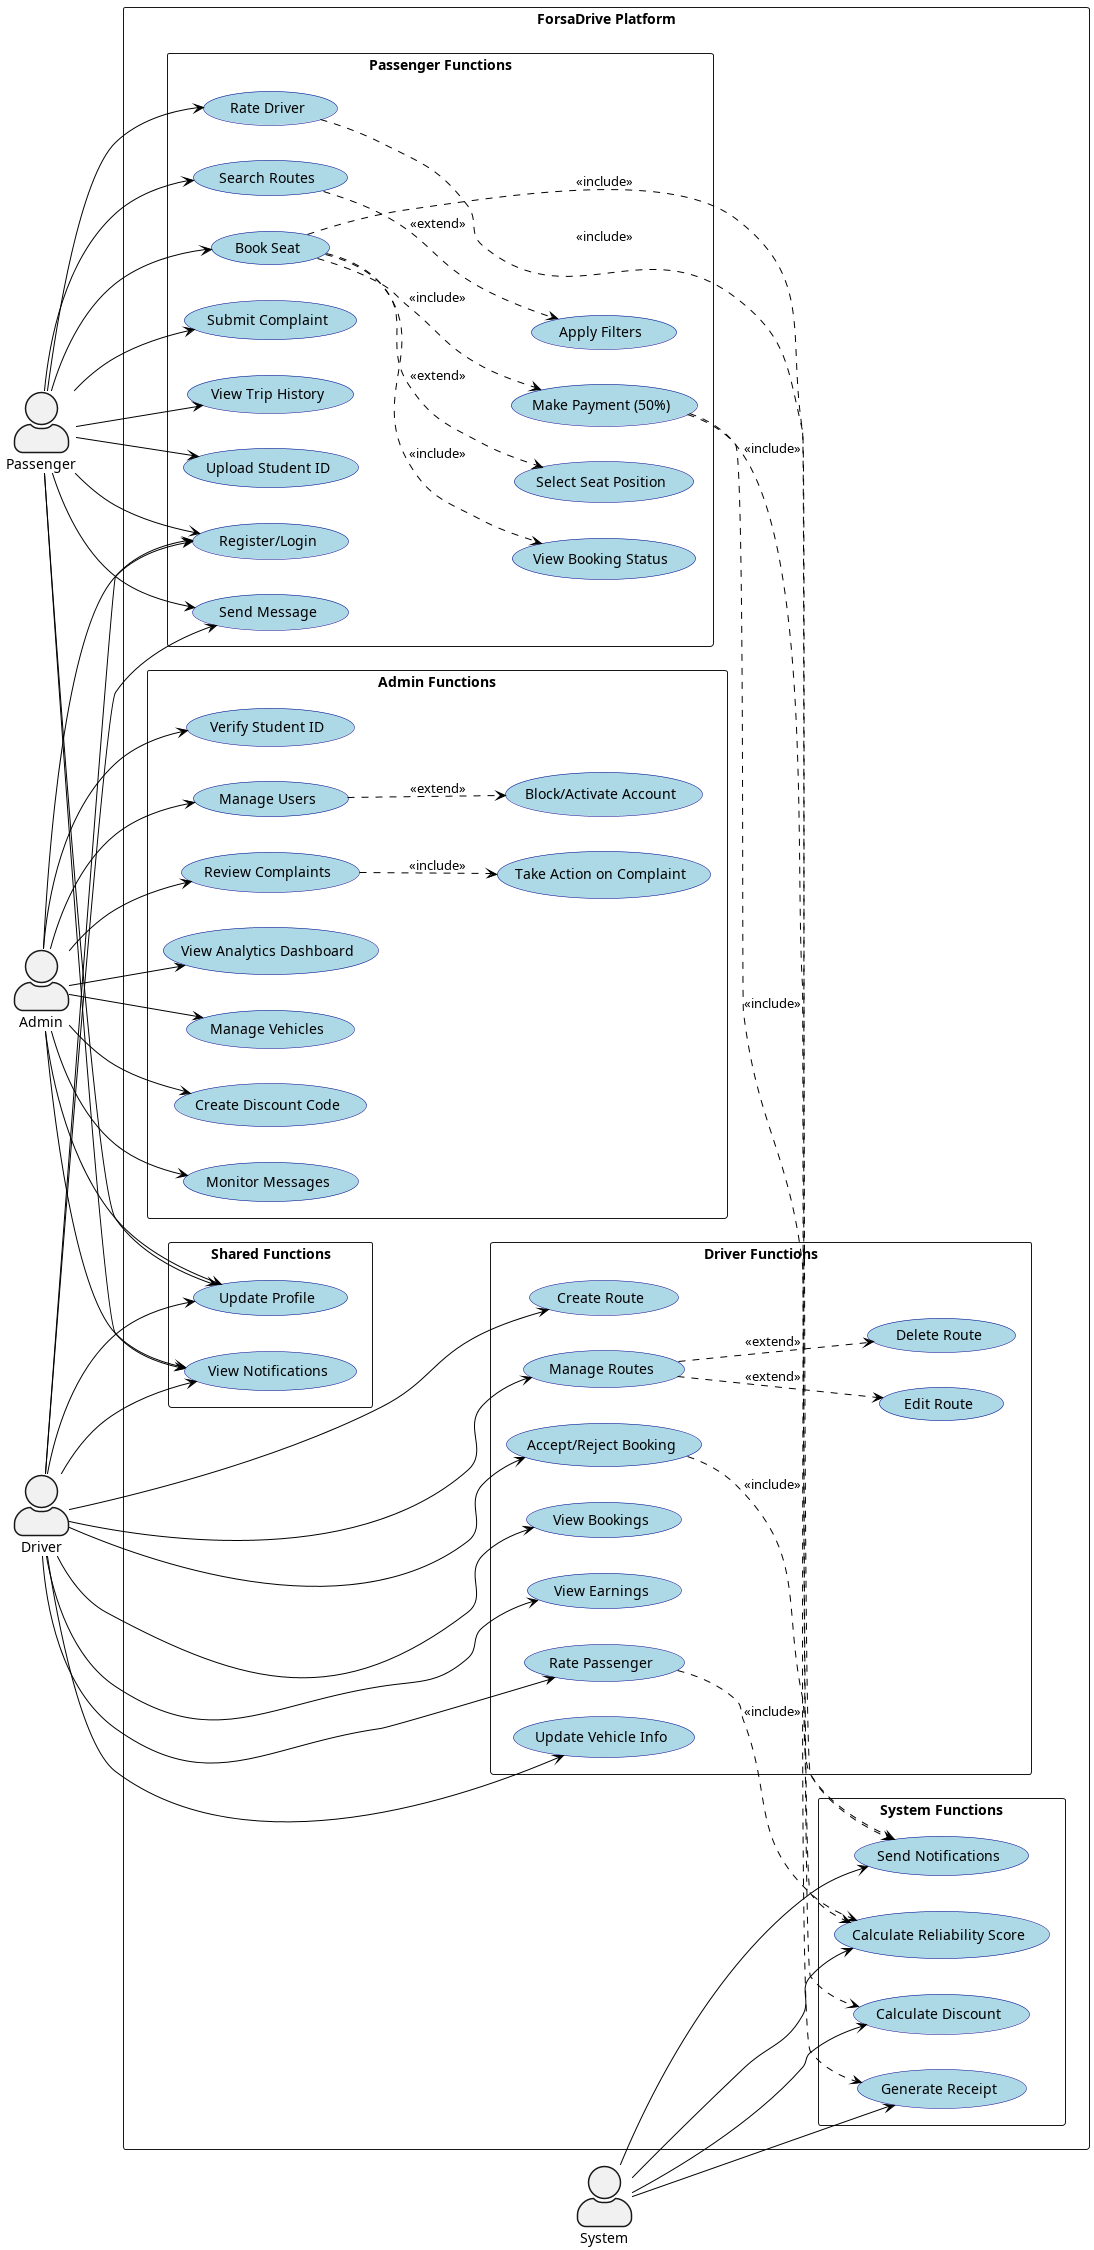
\includegraphics[width=0.7\textwidth]{ForsaDrive_UseCase.png}
    \caption{Global use case diagram of ForsaDrive}
    \label{fig:global_use_case}
\end{figure}


\section*{Conclusion}

This chapter defined the functional scope of ForsaDrive. The comparative study of existing solutions confirmed the absence of a carpooling platform genuinely adapted to the Tunisian context and clarified the gap that the project aims to fill. The presentation of the Scrum methodology and its concrete application to a four-sprint plan introduced the rhythm under which the work was carried out. The identification of the actors and the listing of the functional and non-functional requirements then translated the high-level objectives of the project into a precise specification, which is summarized in the global use case diagram. The next chapter takes this specification as input and produces a detailed conception of the platform, covering its architecture, the dynamic behavior of its most representative scenarios, and the structure of its data.